% Metódy inžinierskej práce

\documentclass[10pt,slovak,a4paper]{article}
\usepackage[slovak, english]{babel}
\usepackage[IL2]{fontenc} 
\usepackage[utf8]{inputenc}
\usepackage{graphicx}
\usepackage{url}
\usepackage{hyperref} 
\graphicspath{{imgs/}}
\usepackage{cite} 
\usepackage{tabularx}


\pagestyle{headings}

\title{Describing the capabilities and cases of uses for sequence diagrams in software engineering \thanks{Semestrálny projekt v predmete Metódy inžinierskej práce, ak. rok 2021/22, vedenie: Shevchenko Serhii}} % meno a priezvisko vyučujúceho na cvičeniach

\author{Shevcheko Serhii\\[2pt]
	{\small Slovenská technická univerzita v Bratislave}\\
	{\small Fakulta informatiky a informačných technológií}\\
	{\small \texttt{xshevchenko@stuba.sk}}
	}

\date{\small 5. november 2021} 



\begin{document}

\maketitle

\begin{abstract}
The article will describe the general principles of constructing sequence diagrams, and provide optimal cases of their use in the field of software engineering modeling.

The main structural elements of a sequence diagram will be described, the rules for their use with corresponding examples.
\end{abstract}



\section{Introduction}

In the well-known graphical description language for modeling in the field of software development, UML, there are several types of diagrams, each of which has its own advantages and disadvantages.

Among the popular types of diagrams are class diagrams, component diagrams, and activity diagrams.

The problem with all the above diagrams is that they cannot simulate the dynamics of the model, the behavior and the relationship between "actors" over time. They represent the structure, but not the behavior of the model on the timeline.

To solve this problem, a sequence diagram was created. It, unlike other types of diagrams, shows the interactions of "actors" on the timeline, the exchange of "messages" (data) between them. And, again, this is all shown in projection on the time axis. That is, it allows to explore the model in dynamics~\cite{Sequence_diagram:Lambert}.

\section{What is UML?} \label{what_is_diagram}
Before we talk about sequence diagrams, we should first understand what UML is, of which the sequence diagram is a part.

The Unified Modeling Language (UML) is a general-purpose, developmental, modeling language in the field of software engineering that is intended to provide a standard way to visualize the design of a system~\cite{UML_Distilled}. 

In other words, we can say that UML is a set of rules and recommendations on how to create visual structural and relational models of software systems.

The creation of UML was originally motivated by the desire to standardize the disparate notational systems and approaches to software design. It was developed at Rational Software in 1994–1995, with further development led by them through 1996~\cite{UML_user_guide:Booch}.

\subsection{What UML include?}
The fact is UML consist of many types of diagrams \ref{UML:diagrams}. In order to understand the benefits of a sequence diagram, it is important first to understand what other diagrams exist in UML and for what purposes they are used.

\begin{figure*}[tbh]
	\centering
	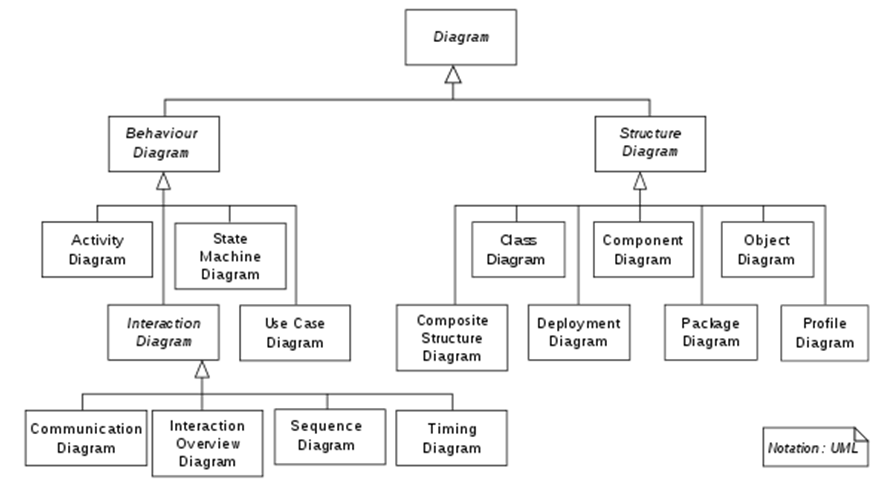
\includegraphics[scale=0.5]{UML diagrams.png}
	\caption{Diagram types \cite{UML_user_guide:Booch}.}
	\label{UML:diagrams}
	\end{figure*}

Looking at Figure \ref{UML:diagrams}, we see that the structural tree of UML diagrams is rather voluminous. Not all of these diagrams are actively used in the development industry ~\cite{UML_Distilled}, but each was created for a specific purpose. In Table 1, we can see the 4 main types of diagrams actively used in the development industry, and a short summary of their purpose and structural composition.

 \begin{table}[htbp]
	\begin{tabular}{|p{0.35\linewidth}|p{0.35\linewidth}|p{0.35\linewidth}|}
	\hline
					  & Uses for representation                                                          & Consist of                                    \\ 
					  \hline
	Sequence diagram  & relations of the object in time sequence                                         & objects and messages on lifeline.             \\ 
	\hline
	Class diagram     & static classes structure in a model and relations between them.                  & classes, that contain attributes and methods. \\ 
	\hline
	Activity diagram  & of workflows of stepwise activities and actions.                                 & activities and logic blocks.                  \\ 
	\hline
	Component diagram & how components are wired together to form larger components or software systems. & structural components.                        \\ 
	\hline
	\end{tabular}
\end{table}

\section{When to use a sequence diagram} \label{when}
A sequence diagram should be used primarily to visualize relationships between objects, taking into account the sequence of these very relationships~\cite{IBM_SD}.

This diagram is very useful for modeling synchronous services, it allows you to think through all the interactions between "actors" from the beginning to the end of the service life cycle on the timeline.
% Z obr.~\ref{f:rozhod} je všetko jasné. 

\begin{figure*}[tbh]
\centering
%\includegraphics[scale=1.0]{diagram.pdf}
% Aj text môže byť prezentovaný ako obrázok. Stane sa z neho označný plávajúci objekt. Po vytvorení diagramu zrušte znak \texttt{\%} pred príkazom \verb|\includegraphics| označte tento riadok ako komentár (tiež pomocou znaku \texttt{\%}).
% \caption{Rozhodujúci argument.}
% \label{f:rozhod}
\end{figure*}

\section{The notation} \label{notation}

% Základným problémom je teda\ldots{} Najprv sa pozrieme na nejaké vysvetlenie (časť~\ref{ina:nejake}), a potom na ešte nejaké (časť~\ref{ina:nejake}).\footnote{Niekedy môžete potrebovať aj poznámku pod čiarou.}

% Môže sa zdať, že problém vlastne nejestvuje\cite{Coplien:MPD}, ale bolo dokázané, že to tak nie je~\cite{Czarnecki:Staged, Czarnecki:Progress}. Napriek tomu, aj dnes na webe narazíme na všelijaké pochybné názory\cite{PLP-Framework}. Dôležité veci možno \emph{zdôrazniť kurzívou}.


\subsection{Frame} \label{notation:frame}
The first notation element to know is the frame. It is makes a graphical boundary of a sequence diagram and provide place for a diagram label (Frame \ref{fig:frame}). 
\begin{figure*}[tbh]
\centering
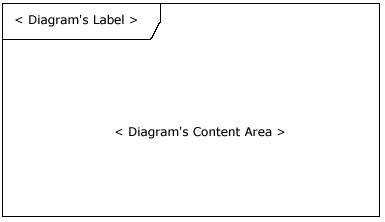
\includegraphics[scale=0.5]{frame.jpg}
\caption{Frame template.}
\label{fig:frame}
\end{figure*}

This element is not required in sequence diagrams, but it is better to use it for convenience. When using this element, it is necessary to place all subsequent elements, which will be described below, inside the frame.

\subsection{Lifelines} \label{notation:lifelines}
Lifelines are designations of objects that make up the model, and between which information is exchanged. This is one of the key elements of a sequence diagram.
\begin{figure*}[tbh]
	\centering
	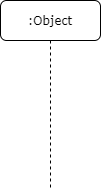
\includegraphics[scale=0.6]{lifeline.png}
	\caption{Lifeline template.}
	\label{fig:lifeline}
\end{figure*}

Lifelines are drawn as a box with a dashed line descending from the center of the bottom edge (Figure \ref{fig:lifeline})\cite{IBM_SD}.


\subsection{Messages} \label{notation:messages}
Messages are illustrating calling a function from one object to another, data exchange between the objects.
\begin{figure*}[tbh]
	\centering
	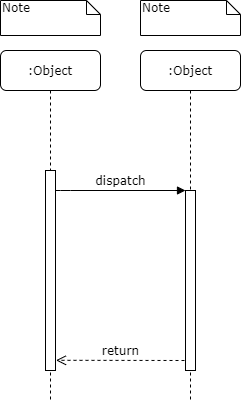
\includegraphics[scale=0.6]{Message.png}
	\caption{Messages template.}
	\label{fig:messages}
\end{figure*}
There are dispatch messages, that display calling functions, and return message, that display end of execution\cite{UML}.

White rectangle is an Execution Specification, it is used to visually display the start and end of an operation.
\section{Building a Sequence Diagram} \label{building}





\section{Conclusion} \label{Conclusion} % prípadne iný variant názvu






% týmto sa generuje zoznam literatúry z obsahu súboru literatura.bib podľa toho, na čo sa v článku odkazujete
\bibliography{literatura}
\bibliographystyle{plain} % prípadne alpha, abbrv alebo hociktorý iný
\end{document}
